
%(BEGIN_QUESTION)
% Copyright 2011, Tony R. Kuphaldt, released under the Creative Commons Attribution License (v 1.0)
% This means you may do almost anything with this work of mine, so long as you give me proper credit

Determine the direction of this controller's action (either {\it direct} or {\it reverse}) based on an analysis of its programming code:

$$\includegraphics[width=15.5cm]{i00896x01.eps}$$

\hbox{ \vrule
\vbox{ \hrule \vskip 3pt
\hbox{ \hskip 3pt
\vbox{ \hsize=5in \raggedright

\noindent
\underbar{\bf Pseudocode listing}

{\tt Declare Pin0 as an analog input (scale 0 to 5 volts = 0 to 1023)}

{\tt Declare Pin1 as an analog output (scale 0 to 5 volts = 0 to 1023)}

{\tt Declare SP as a variable, initially set to a value of 614}

{\tt Declare GAIN as a variable, initially set to a value of 1.0}

{\tt Declare ERROR as a variable}

{\tt Declare BIAS as a variable, initially set to a value of 614}

\vskip 10pt

{\tt LOOP}

\hskip 10pt {\tt SET ERROR = SP - Pin0}

\hskip 10pt {\tt SET Pin1 = (GAIN * ERROR) + BIAS}

{\tt ENDLOOP}
}
\hskip 3pt}%
\vskip 5pt \hrule}%
\vrule}

\vskip 10pt

Now, assuming you cannot change the programming code -- but only the values of the {\tt GAIN} and {\tt BIAS} variables, and the electrical connections to the controller -- determine a way to switch the controller's action to the opposite direction. 

\underbar{file i00896}
%(END_QUESTION)





%(BEGIN_ANSWER)

I recommend 5 points for the correct action, and 5 points for a workable solution:

\vskip 10pt

The action as programmed is {\bf reverse}.  In order to make the action direct, you may enter a negative value instead of a positive value for {\tt GAIN}.

%(END_ANSWER)





%(BEGIN_NOTES)

{\bf This question is intended for exams only and not worksheets!}.

%(END_NOTES)


